\chapter{Game Design}
For this thesis work I designed and implemented a game called Space-run, which involves attempting to accumulate the highest score possible by navigating through three distinct tunnels while avoiding various obstacles. The game is endless in nature, as the speed increases each time the player successfully completes all three tunnels. 

It is worth noting that, in designing this game, I was inspired by the pre-existing Tunnel Rush (\cite{tunnelrush}). Tunnel Rush and Space-run are both 3D tunnel games that involve advancing through a tunnel to avoid traps. However, there are several key differences between the two games. Tunnel Rush is a web-based game played in first-person perspective, while Space-run is a desktop-based game played in third-person perspective. Tunnel Rush has levels, some of which are inverted with the traps on top of the tunnel and the player outside of it. Space-run, since inspired by Tunnel Rush, also has levels, but they are all inside the tunnel and features not only traps but also creatures that the player must avoid or shoot. Additionally, Space-run has a computer-themed setting, with elements such as battery, bugs, and viruses.

\section{Player and Movement}

\begin{figure}[h]
    \centering
    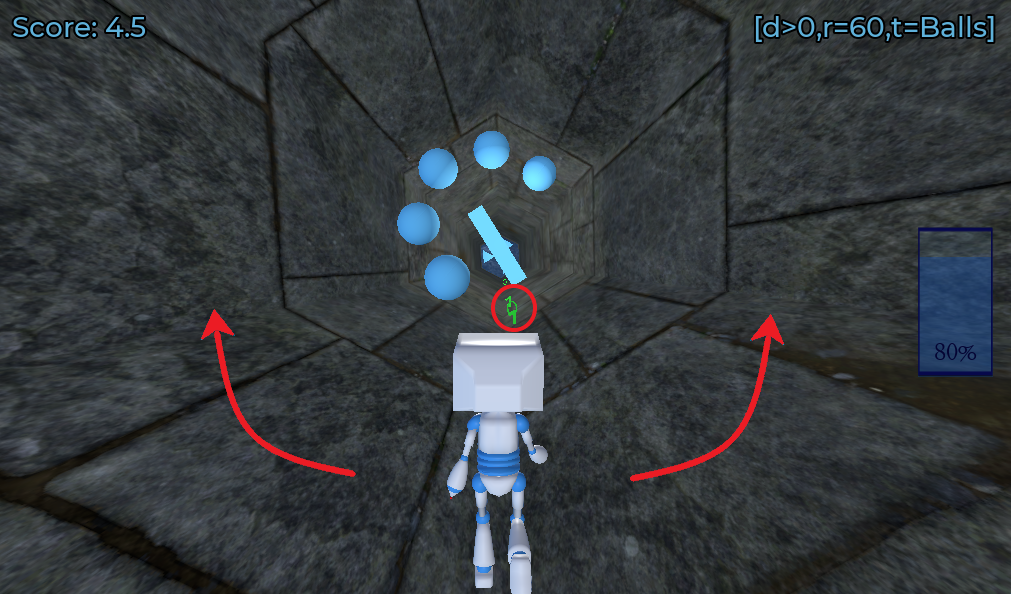
\includegraphics[width=\textwidth]{second_tunnel}
    \caption{Movement}
    \label{fig:snd_tunnel}
\end{figure}

In Space-run the player assumes control of a character named Hans (see Figure \ref{fig:hans}) who continually advances at a constant speed through the tunnels. To navigate through the game, the player must use the left and right arrow keys to rotate the current tunnel and avoid obstacles (as shown in Figure \ref{fig:snd_tunnel}). 
\begin{wrapfigure}{r}{0.25\textwidth}
    \centering
    
\includegraphics[scale=0.6]{hans}
    \caption{Hans}
    \label{fig:hans}
\end{wrapfigure}
In addition to these lateral movements, Hans also has the ability to shoot bullets (also shown in Figure \ref{fig:snd_tunnel}) by pressing the space key, which can be used to defeat certain in-game creatures and earn a higher score. The player must utilize these abilities in order to progress through the game and achieve a high score.

\section{Obstacles}
As previously stated, the player must navigate through various obstacles in the game. These obstacles can be divided into three distinct categories, and each tunnel contains a unique subset of them. In the subsequent sections, we will delve deeper into these categories in order to better understand the challenges faced by the player.

\subsection{Traps}
\begin{figure}[h]
    \centering
    
\includegraphics[width=\textwidth]{traps}
    \caption{Trap examples}
    \label{fig:traps}
\end{figure}
As depicted in Figure \ref{fig:traps}, a selection of the various trap types that the character Hans must avoid is presented. These traps, of which there are a total of 10, vary in their level of difficulty and can be either static or animated. They traps can be encountered in any of the three tunnels, and if the player fails to successfully evade them, they result in an instant death.

\subsection{Bugs}
\label{Bugs}
\begin{figure}[h]
    \centering
    
\includegraphics[width=\textwidth]{bugs}
    \caption{Bugs}
    \label{fig:bugs}
\end{figure}
In addition to traps, the game also features bugs as an obstacle (as shown in Figure \ref{fig:bugs}). The bugs appear in the second tunnel and are designed to rotate around the tunnel toward the player's position, making them more challenging to evade. However, it is still possible to avoid them. If the player chooses to engage with the bugs, they can be defeated by shooting three bullets at them. If the player collides with a bug, Hans will lose 25\% of his battery life (for more information on battery life, see Section \ref{AdditionalFeatures}).

\subsection{Viruses}
\begin{figure}[h]
    \centering
    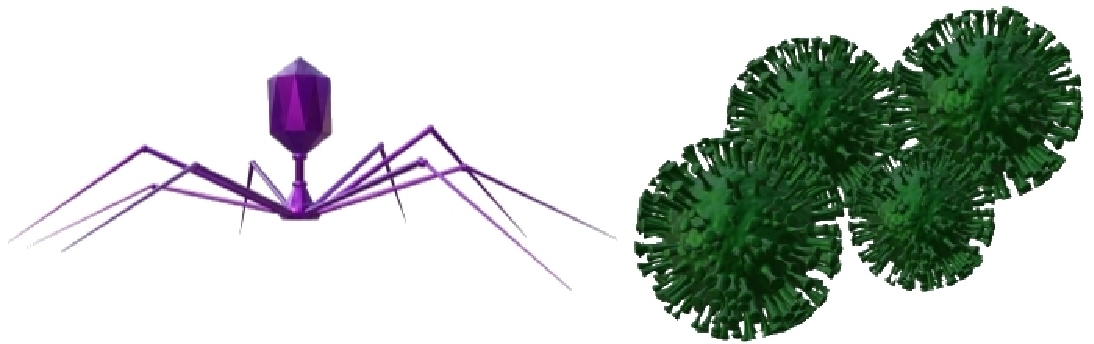
\includegraphics[width=\textwidth]{viruses}
    \caption{Bacteriophage and Rotavirus}
    \label{fig:viruses}
\end{figure}

The third and final type of obstacle in the game are viruses (illustrated in Figure \ref{fig:viruses}). These viruses are found in the third tunnel and, similar to bugs, can be eliminated through the use of three bullets. They also, just like bugs, rotate around the tunnel toward the player's position. Bacteriophage, a subtype of virus, will result in an instant death if the player comes into contact with them. Rotaviruses, on the other hand, will cause the player's character to become sick for a brief period of time. During this illness, it is crucial for the player to avoid coming into contact with another Rotavirus, as this will result in the end of the game.

\section{Additional Features}
\label{AdditionalFeatures}
\begin{figure}[h]
    \centering
    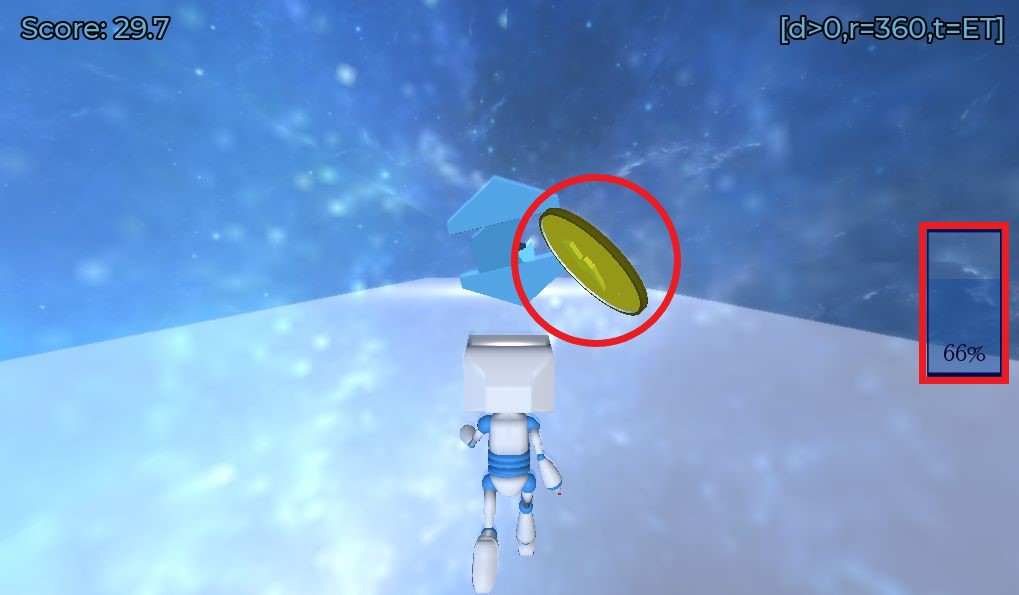
\includegraphics[width=\textwidth]{first_tunnel}
    \caption{Battery and Energy Token}
    \label{fig:batteryToken}
\end{figure}

There are several other features of the game that are worth mentioning. One of the most significant of these is the battery life of the player's character, Hans, which is displayed on the right side of the screen (as shown in Figure \ref{fig:batteryToken}). As Hans is designed to resemble a computer, it is necessary for him to recharge his battery throughout the game by collecting energy tokens (Figure \ref{fig:batteryToken}). This will fully restore his battery capacity. There are three main ways in which Hans can lose battery life: running causes a constant reduction of 1\% every 0.5 seconds, each bullet shot costs 1\% of the battery life, and coming into contact with a bug results in a reduction of 25\% (as described in Section \ref{Bugs}). If the battery reaches 0\%, Hans will die and the game will end.

Finally, it should be noted that upon successfully navigating through all three types of tunnels, the game will increase in speed and the player will once again encounter the same tunnels, looping through them indefinitely until the player loses.

\section{Score Count and Winning}
The score of the game is based on the length of time that the player is able to survive. Additionally, each time a player successfully shoots down a bug or virus, their score increases by 10 points. As previously mentioned, the game is designed to be played indefinitely, but for the purpose of this study, we have set the game to be considered won after an agent successfully completes nine tunnels, reaching level 15.
